\documentclass[archE1,portrait]{baposter}

% ---------------------------------------------------------
% Paquetes básicos
% ---------------------------------------------------------
\usepackage[utf8]{inputenc}
\usepackage[T1]{fontenc}
\usepackage[spanish]{babel}
\usepackage{amsmath, amssymb}
\usepackage{graphicx}
\usepackage{booktabs}
\usepackage{caption}
\usepackage{url}
\usepackage[hidelinks]{hyperref}
\usepackage{multicol}
\usepackage{wrapfig}

% ---------------------------------------------------------
% Configuración de colores
% ---------------------------------------------------------
\definecolor{bordercol}{RGB}{5,2,82}
\definecolor{headercol1}{RGB}{30,64,120}
\definecolor{headercol2}{RGB}{30,64,120}
\definecolor{headerfontcol}{RGB}{255,255,255}
\definecolor{boxcolor}{RGB}{245,245,255}

\renewcommand{\familydefault}{\sfdefault} % Sans serif moderno

\begin{document}

\begin{poster}{
    grid=false,
    borderColor=bordercol,
    headerColorOne=headercol1,
    headerColorTwo=headercol2,
    headerFontColor=headerfontcol,
    boxColorOne=boxcolor,
    headershape=roundedright,
    headerfont=\Large\sf\bf,
    textborder=rectangle,
    background=user,
    headerborder=open,
    boxshade=plain
}
%
% ---------------------------------------------------------
% TÍTULO Y AUTORES
% ---------------------------------------------------------
%
{\sf\bfseries Explorando sistemas cuánticos con Python: una introducción computacional para el aula moderna}
{\vspace{1em}
\textbf{Rafael Obed Egurrola Corella}, \textit{Asesor: Nombre del Asesor} \\[0.3em]
{\small Departamento de Física, Universidad de Sonora} \\[-0.3em]
\href{mailto:a220211866@unison.mx}{a220211866@unison.mx}}
{
\includegraphics[width=0.15\linewidth]{logo_unison}}

% ---------------------------------------------------------
% INTRODUCCIÓN Y MOTIVACIÓN
% ---------------------------------------------------------
\headerbox{Introducción y Motivación}{name=intro,column=0,row=0,span=3}{
La enseñanza tradicional de la mecánica cuántica suele centrarse en soluciones analíticas de sistemas idealizados (pozos infinitos, osciladores armónicos, átomos de hidrógeno).  
Sin embargo, la práctica moderna de la física se apoya fuertemente en métodos computacionales para explorar sistemas más complejos y realistas.

\vspace{1em}
Este proyecto desarrolla una \textbf{librería educativa en Python} que permite a los estudiantes resolver la ecuación de Schrödinger para distintos sistemas y visualizar sus soluciones.  
El objetivo es \textit{integrar la simulación numérica como herramienta pedagógica} que refuerce la comprensión conceptual, promueva la experimentación y fomente el pensamiento computacional.

\vspace{0.8em}
\begin{center}
\textit{“Lo que no se puede simular, no se comprende del todo.”}
\end{center}
}

% ---------------------------------------------------------
% METODOLOGÍA Y HERRAMIENTAS
% ---------------------------------------------------------
\headerbox{Metodología y Herramientas}{name=methods,column=0,below=intro,span=3}{

\begin{minipage}[t]{0.48\linewidth}
\vspace{0pt}
\underline{\textbf{Librería Computacional en Python}}
\begin{itemize}
    \item \textbf{Código abierto:} Implementado en Python con NumPy, SciPy y Matplotlib. El repositorio está disponible en GitHub para promover el aprendizaje colaborativo.
    \item \textbf{Módulo \texttt{numerov.py}:} Implementa el método de Numerov para resolver la ecuación de Schrödinger unidimensional.
        \begin{itemize}
            \item Aplicaciones: oscilador armónico, parte radial del átomo de hidrógeno.
        \end{itemize}
    \item \textbf{Módulo \texttt{hartreefock.py}:} Implementa el método de Hartree–Fock mediante el esquema SCF para sistemas multielectrónicos simples.
        \begin{itemize}
            \item Aplicaciones: moléculas $\text{H}_2$, $\text{HeH}^+$.
        \end{itemize}
    \item \textbf{Visualización:} Generación de funciones de onda, densidades de probabilidad y espectros energéticos.
\end{itemize}
\end{minipage}
\hfill
\begin{minipage}[t]{0.48\linewidth}
\vspace{0pt}
\underline{\textbf{Marco Pedagógico: Taxonomía de Bloom}}
\begin{itemize}
    \item Nuestra propuesta busca guiar a los estudiantes a través de los niveles cognitivos superiores de la taxonomía de Bloom:
    \begin{itemize}
        \item \textbf{Aplicar:} Resolver problemas con los módulos del código.
        \item \textbf{Analizar:} Interpretar gráficas y comparar con soluciones analíticas.
        \item \textbf{Evaluar:} Discutir precisión y limitaciones de los métodos numéricos.
        \item \textbf{Crear:} Modificar el código para explorar nuevos potenciales o moléculas.
    \end{itemize}
    \item Este enfoque promueve la autonomía, la curiosidad y la transferencia de conocimiento.
\end{itemize}
\end{minipage}
}

% ---------------------------------------------------------
% RESULTADOS Y APLICACIONES
% ---------------------------------------------------------
\headerbox{Resultados y Aplicaciones}{name=results,column=0,below=methods,span=2}{
La librería permite obtener representaciones gráficas directas de conceptos cuánticos abstractos.  
Todos los resultados mostrados fueron generados íntegramente con nuestro código.

\begin{center}
\begin{minipage}[c]{0.48\linewidth}
    \centering
    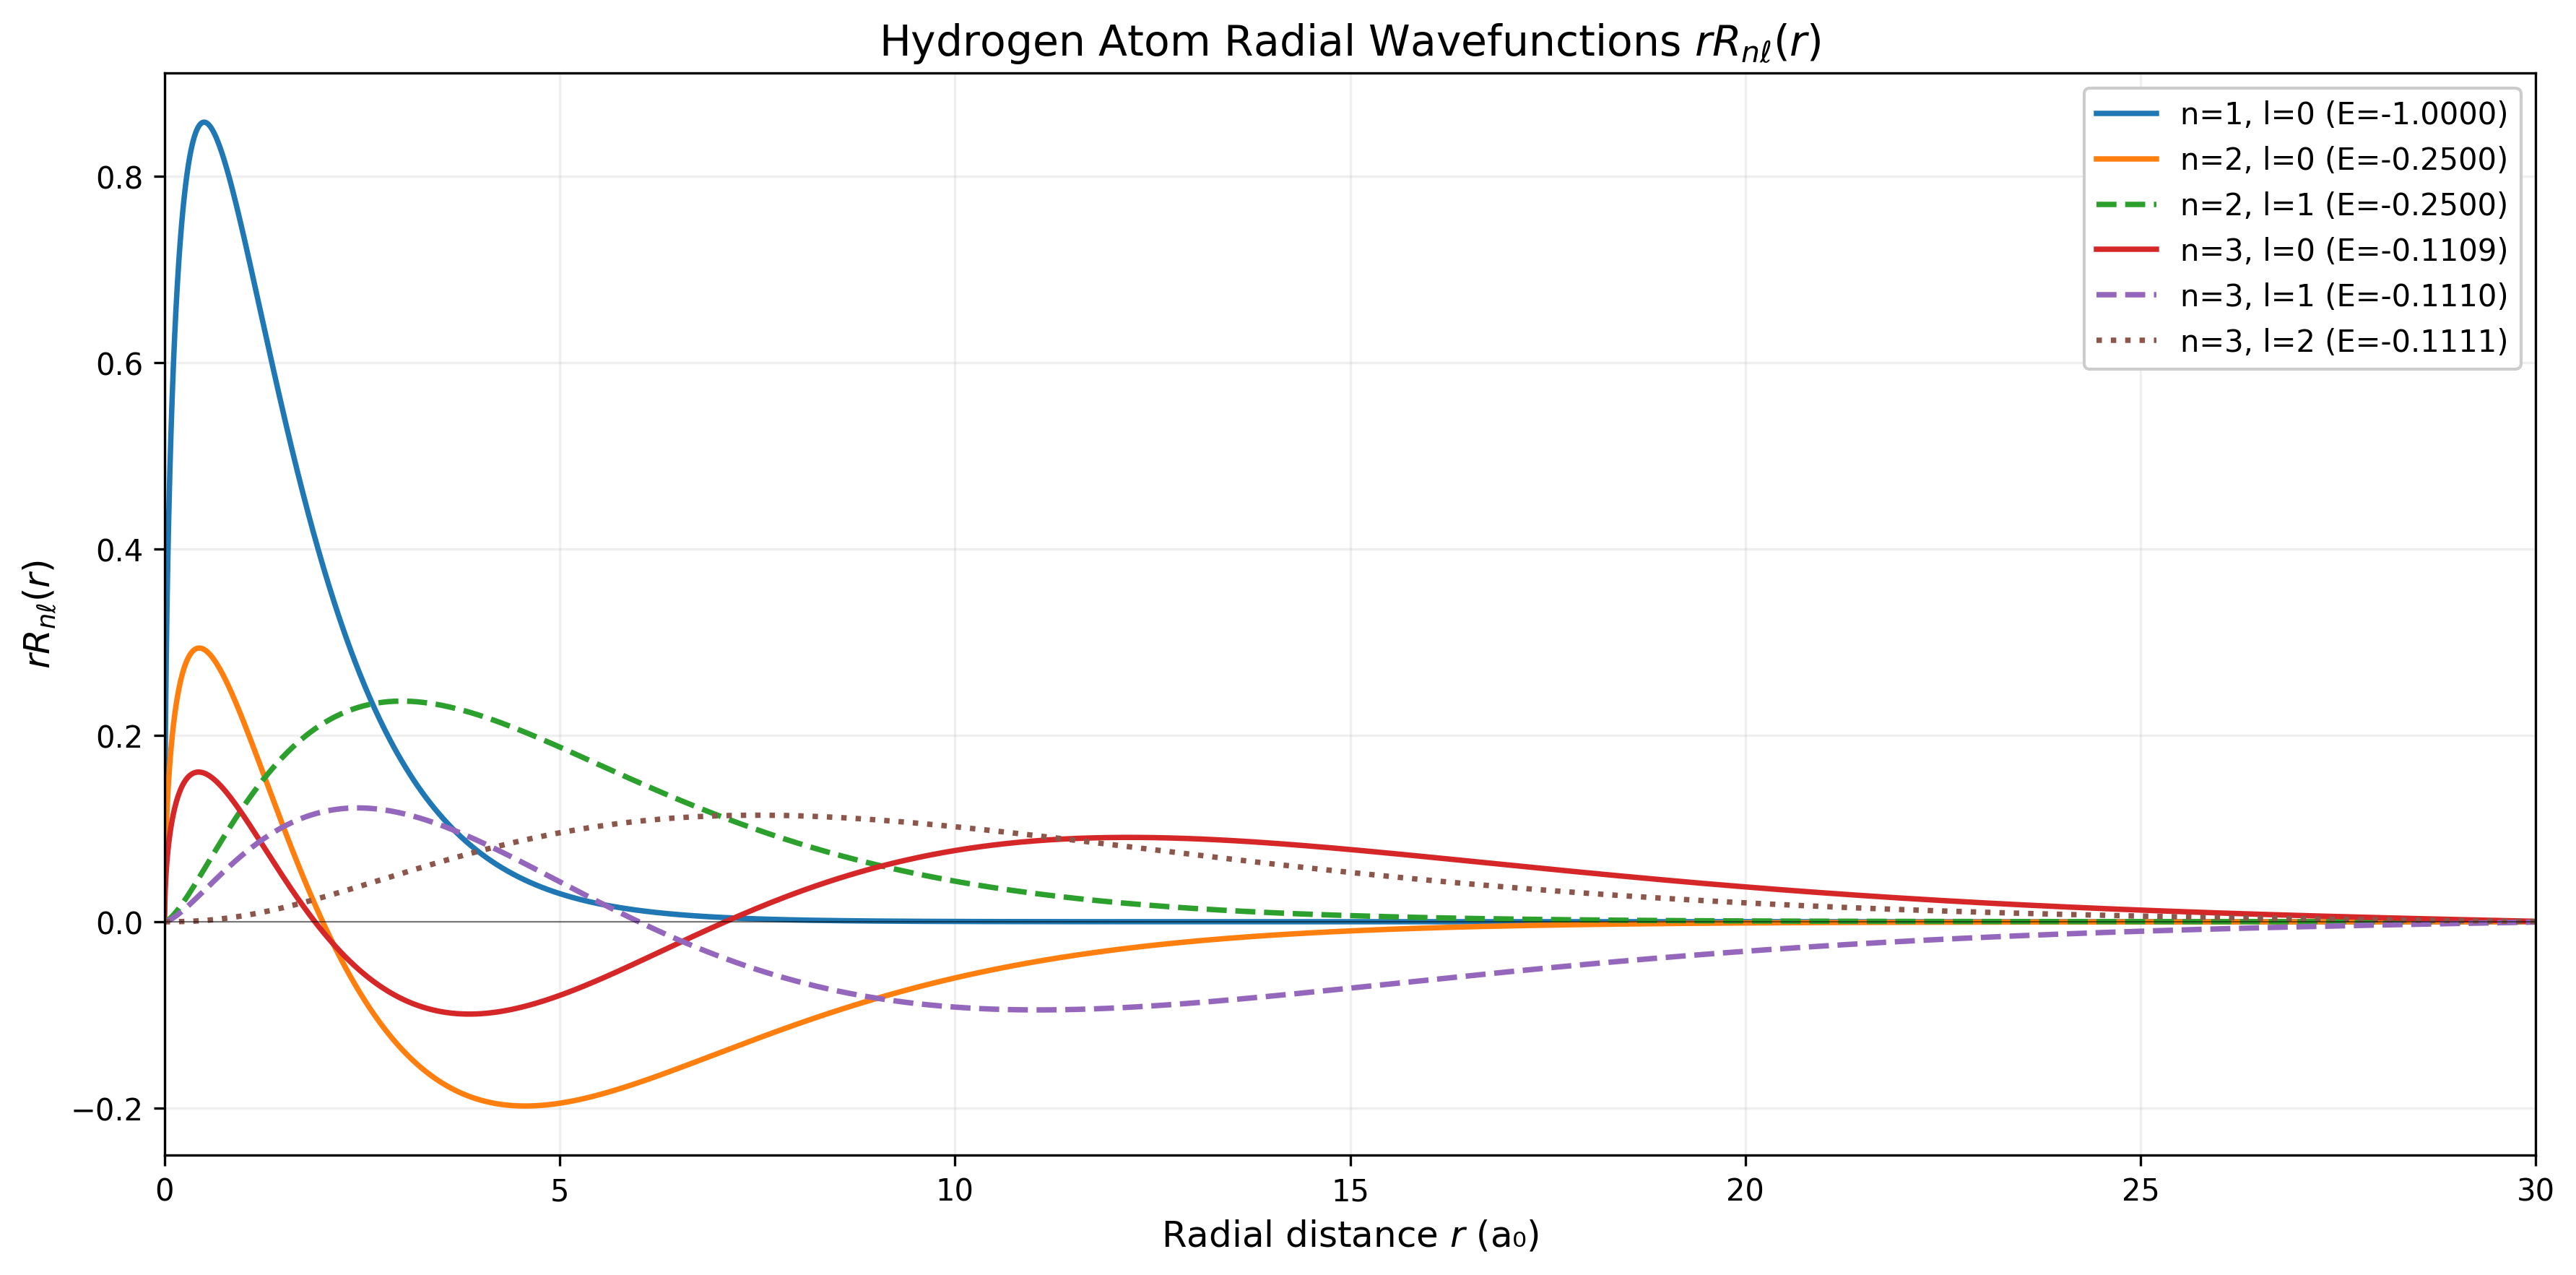
\includegraphics[width=0.9\linewidth]{hydrogen.png}
    \captionof{figure}{Funciones radiales $R_{n0}(r)$ del átomo de hidrógeno.}
\end{minipage}\hfill
\begin{minipage}[c]{0.48\linewidth}
    \centering
    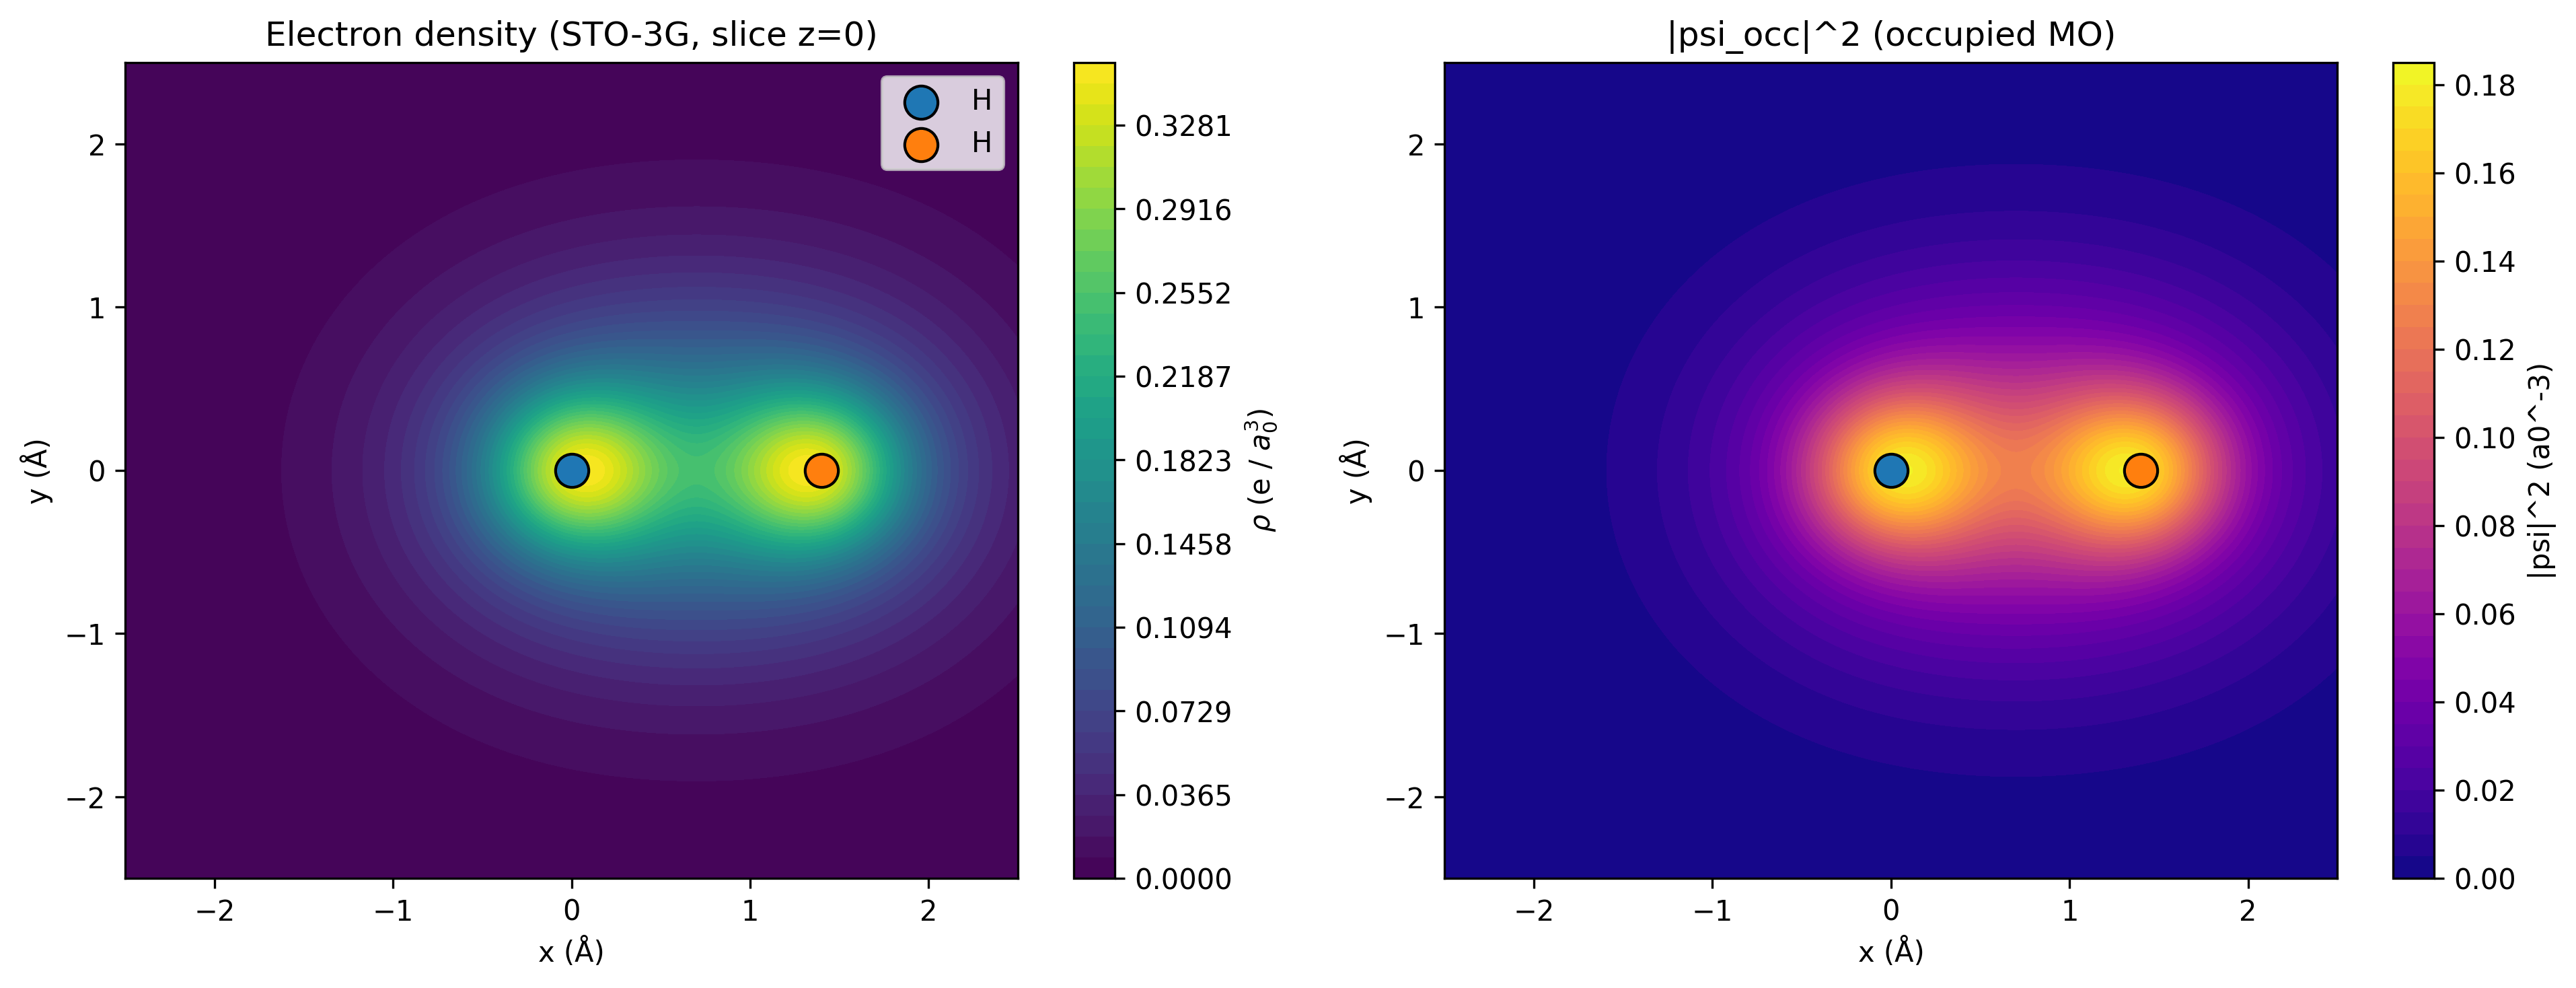
\includegraphics[width=0.9\linewidth]{hf_h2.png}
    \captionof{figure}{Densidad de probabilidad electrónica para la molécula de $\text{H}_2$.}
\end{minipage}
\end{center}

\vspace{0.5em}
Los estudiantes pueden extender el código para estudiar potenciales dependientes del tiempo o modelos de confinamiento cuántico, acercándose a prácticas de investigación reales.
}

% ---------------------------------------------------------
% CONCLUSIONES
% ---------------------------------------------------------
\headerbox{Conclusiones y Trabajo Futuro}{name=conclusion,column=2,below=methods,span=1}{
\begin{itemize}
    \item La simulación numérica en Python es una herramienta poderosa para el aprendizaje activo de la física cuántica.
    \item Nuestro enfoque permite que los estudiantes visualicen la teoría, experimenten con parámetros y construyan intuición física.
    \item Futuro: Extensión del código hacia métodos post-Hartree–Fock y potenciales dependientes del tiempo.
    \item El proyecto busca consolidarse como un recurso abierto para la docencia en física computacional.
\end{itemize}
}

% ---------------------------------------------------------
% REFERENCIAS
% ---------------------------------------------------------
\headerbox{Referencias}{name=references,column=2,below=conclusion}{
\smaller
\bibliographystyle{apalike}
\bibliography{referencias}
}

% ---------------------------------------------------------
% PIE / ENLACE
% ---------------------------------------------------------
\headerbox{}{name=footer,column=0,span=3,below=results}{
\centering
\small
Código y documentación disponibles en: \url{https://github.com/tuusuario/cuanticapy}
}

\end{poster}
\end{document}
